\newpage

\section{Attualizzazione dei rischi} \label{RiscontroRischi}

Vengono di seguito analizzati i problemi riscontrati durante lo svolgimento del progetto, suddivisi per ogni periodo; ad ogni occorrenza rilevata corrisponderà una breve descrizione del problema e le contromisure adottate per la sua mitigazione. È inoltre possibile prendere visione di come i problemi qui analizzati abbiano influito sul consuntivo di periodo sul preventivo finale nell'\hyperref[ConsuntivoPeriodo]{Appendice B}.\\

\subsection{Analisi dei requisiti}
\begin{table}[h!]
	\centerline{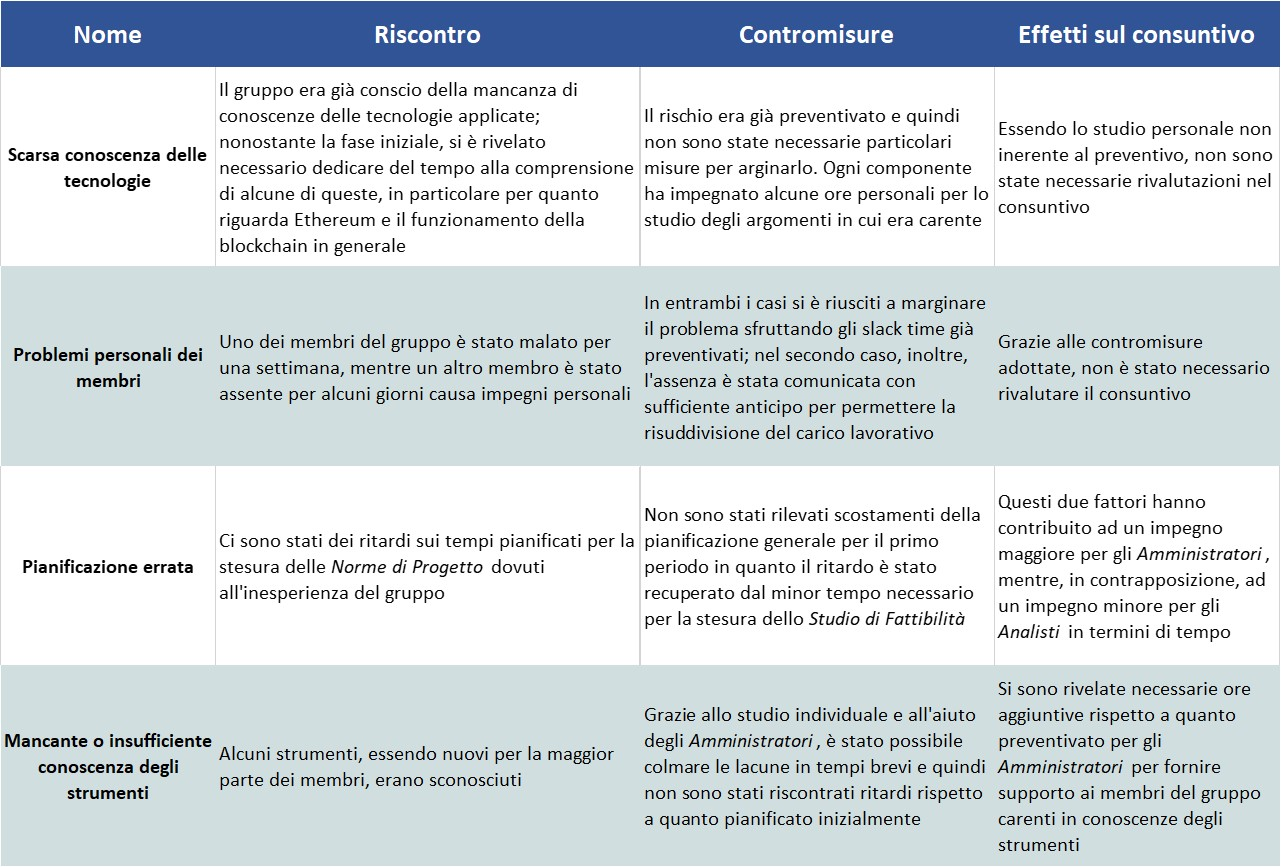
\includegraphics[scale=0.55]{img/Rischi/RiscontroProblemi-AnalisiRequisiti.jpg}}
	\caption{Riscontro problemi: Analisi dei Requisiti}
\end{table}
\clearpage

\subsection{Analisi dei requisiti in Dettaglio} \label{RiscontroAnalisiDettaglio}
\begin{table}[h!]
	\centerline{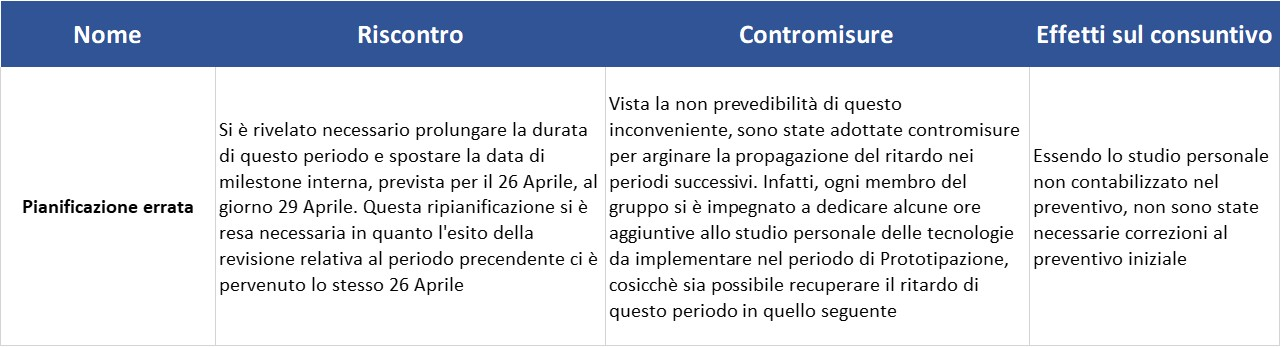
\includegraphics[scale=0.55]{img/Rischi/RiscontroProblemi-AnalisiRequisitiDettaglio.jpg}}
	\caption{Riscontro problemi: Analisi dei Requisiti in Dettaglio}
\end{table}

\subsection{Prototipazione}
\begin{table}[h!]
	\centerline{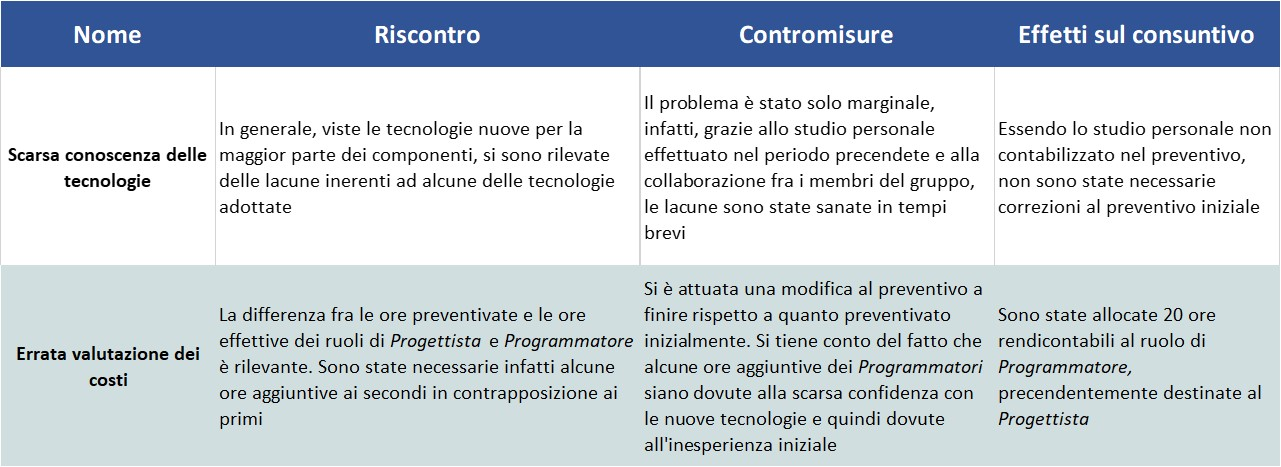
\includegraphics[scale=0.55]{img/Rischi/RiscontroProblemi-Prototipazione.jpg}}
	\caption{Riscontro problemi: Prototipazione}
\end{table}
\clearpage

\subsection{Prototipazione in Dettaglio} \label{RiscontroPrototipazioneDettaglio}
\begin{table}[h!]
	\centerline{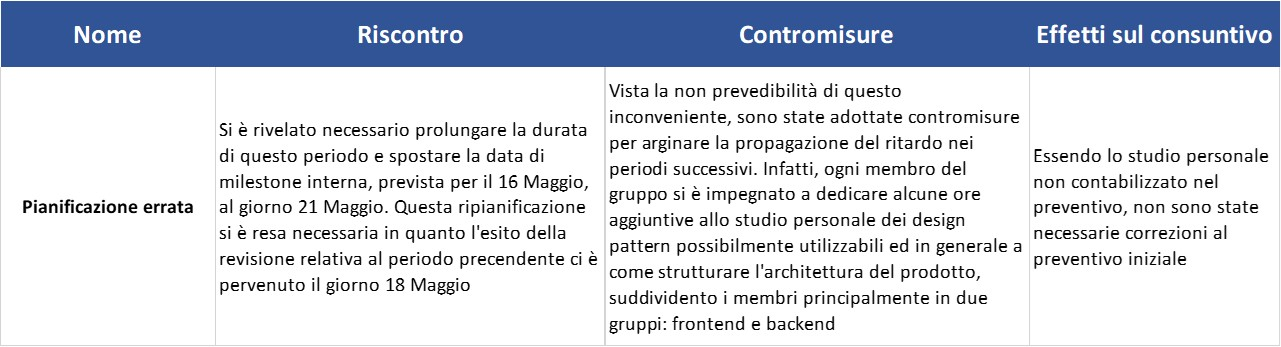
\includegraphics[scale=0.55]{img/Rischi/RiscontroProblemi-PrototipazioneDettaglio.jpg}}
	\caption{Riscontro problemi: Prototipazione in Dettaglio}
\end{table}

\subsection{Progettazione finale e Codifica}
Durante questo periodo non si sono verificati problemi che abbiano influito particolarmente sul perseguimento delle attività pianificate.
